\chapter{Application: Pentagons in Triangle Free Graphs}
\label{chap:pentagon_conjecture}

Given a graph $G$ let $P(G)$ denote the number of pentagons (5-cycles)\footnote{Counted as
subsets: the order does not matter} in $G$.
In 1983 \cite{erdosProblemsGraphTheory1984} Erd\H{o}s made the following conjecture:

\begin{knownconjecture}
    If $G$ is triangle free then $P(G) \leq \left(\frac{|G|}{5}\right)^5$.
\end{knownconjecture}

This conjecture remained open until 2012 when it was proved by both Grzesik
\cite{grzesikMaximumNumberFivecycles2012} and Hatami, Hladký, Králʼ, Norine and Razborov
\cite{hatamiNumberPentagonsTrianglefree2013}. 
Importantly for us, both of these papers used the Razborov flag algebras to prove the result!

\section{The Bounded Degree Conjecture}

Inspired by Erd\H{o}s' conjecture we ask
the following question: Can we bound the number of pentagons in a triangle free graph
as a function of the maximum degree $\Delta(G)$?\footnote{Originally asked by E. Hurley}.
This leads us to the following \textit{bounded degree pentagon conjecture}:

\begin{conjecture}
    \label{conj:bounded_pentagon}
    If $G$ is triangle free then 
    $P(G) \leq \frac{|G|}{5}\left(\frac{\Delta(G)}{2}\right)^4
    =\frac{|G|\Delta(G)^4}{5\cdot 16}$!
\end{conjecture}

\begin{lemma}
    If the bounded degree pentagon conjecture is true then it is tight.
\end{lemma}

\begin{proof}
    Let $k\in\N$ even be given and take $G$ to be the $k/2$-blowup of $C_5$
    (figure \ref{fig:5_partite_graph}) meaning take 5 independent sets of size $k/2$ as
    "supernodes" then densely connect the supernodes into a 5-cycle.
    \begin{figure}[ht]
        \centering
        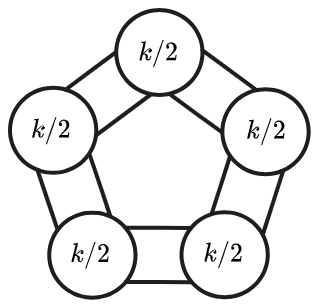
\includegraphics[scale=0.3]{5_partite_graph}
        \caption{Balanced 5-partite cycle graph on $5k/2$ vertices}
        \label{fig:5_partite_graph}
    \end{figure}
    This graph is triangle free: Notice that the induced subgraph on any 3 nodes is bipartite.
    Then we see that choosing
    a vertex from each of the 5 supernodes gives a distinct 5-cycle so there are at
    least $\left(\frac{k}{2}\right)^5$ pentagons in the graph (this is actually exact). But
    $|G|=\frac{5k}{2}$ and $\Delta(G)=k$ so we can rewrite this as
    $\left(\frac{k}{2}\right)^5 = \frac{|G|}{5}\left(\frac{\Delta(G)}{2}\right)^4$ meeting
    the bound. We can do this for any even $k=\Delta(G)$ so this holds asymptotically.
\end{proof}

We claim then the following theorem:
\begin{theorem}
    \label{thm:full_pentagon_bound}
    If $G$ is triangle free then
    $P(G) \leq 0.02073 \cdot |G|\Delta(G)^4 \approx 1.658\frac{|G|}{5}\frac{\Delta(G)^4}{16}$.
\end{theorem}

We prove this result using local flags, but the approach is slightly too complex to serve
as the "warmup" application, so we first first prove this slightly weaker result:

\begin{theorem}
    \label{thm:simple_pentagon_bound}
    If $G$ is triangle free then
    $P(G) \leq \frac{|G|}{5}\frac{\Delta(G)^4}{8} = 2\cdot\frac{|G|}{5}\frac{\Delta(G)^4}{16}$.
\end{theorem}

We will show how we proved the stronger result at the end in section
\ref{sec:pentagon_stronger}.

First we argue that proving an asymptotic bound $P(G) \lesssim \lambda|G|\Delta(G)^4$
proves $P(G) \leq \lambda|G|\Delta(G)^4$ for all $G$.
We then argue that it suffices to prove this asymptotic bound only for regular $G$.

\section{Reductions}

First we argue that an asymptotic bound suffices. Essentially, this is true as any small
graph with a high pentagon density can be expanded to arbitrary high degree.
\begin{lemma}
    \label{lemma:pentagon_asymp_suffices}
    If $P(G) \lesssim \lambda|G|\Delta(G)^4$ as $\Delta(G)\to\infty$ for
    $G$ triangle free
    then $P(G) \leq \lambda|G|\Delta(G)^4$ for all triangle free $G$.
\end{lemma}

\begin{proof}
    More precisely our condition states that for any $\Delta$-increasing sequence of
    triangle free graphs $(G_k)_{k\in\N}$ we have
    $\limsup_{k\to\infty} \frac{P(G_k)}{|G|\Delta(G)^4} \leq \lambda$.

    Assume then for sake of contradiction that there exists $G_0$ triangle free
    such that $\frac{P(G_0)}{|G_0|\Delta(G_0)^4} > \lambda$.
    Let $\delta := \frac{P(G_0)}{|G_0|\Delta(G_0)^4}$ and consider the following
    sequence of graphs $(G_k)_{k\in\N}$: Start with $G_0$ and construct
    $G_{i+1}$ from $G_i$ by doubling every vertex of $G_i$, then for every
    $u\sim v$ in $G_i$ connect both copies of $u$ to both copies of $v$.

    \begin{figure}[!ht]
        \centering
        
\includegraphics[scale=1.5]{pentagon_asymp_construction}
    \end{figure}

    Then we have $|G_{i+1}| = 2|G_i|$ and $\Delta(G_i) = 2\Delta(G_{i+1})$ for all
    $i\in\N$. Note also that $G_i$ triangle free implies $G_{i+1}$ triangle free.
    To see this consider assume $G_i$ triangle free and $G_{i+1}$ has a triangle
    $\{u, v, w\}$. As each of $u,v,w$ are connected they must be copies of three
    different nodes from $G_i$. However such copies are connected iff their originals are
    connected so there must be a corresponding triangle in $G_i$ which is a contradiction.
    Hence each $G_i$ is triangle free.

    Take any pentagon in $G_i$. This correspond to $2^5$ pentagons in $G_{i+1}$. Each
    such pentagon in $G_{i+1}$ we get by expanding a $C_5$ in $G_i$ comes from
    some unique pentagon in $G_i$ hence $P(G_{i+1}) \geq 2^5P(G_i)$ for all $i\geq 1$.
    Hence for every $i\in\N$ we have
    \[
        \frac{P(G_i)}{|G_i|\Delta(G_i^4)} \geq
        \frac{(2^5)^i P(G_0)}{2^i|G_0|(2^i\Delta(G_0))^4}
        = \frac{2^{5i} P(G_0)}{2^{5i}|G_0|\Delta(G_0)^4}
        = \delta
    \]
    and in particular
    \[
        \limsup_{k\to\infty}\frac{P(G_k)}{|G_k|\Delta(G_k)^4} \geq
        \liminf_{k\to\infty}\frac{P(G_k)}{|G_k|\Delta(G_k)^4}
        \geq \delta > \lambda
    \]
    but $(G_k)_{k\in\N}$ is a $\Delta$-increasing sequence of triangle free graphs
    so this contradictions our assumption. Hence no such $G_0$ exists.
\end{proof}

Now we show not only is it enough to show this bound asymptotically, it also suffices
to show the bound only for regular graphs.

\begin{lemma}
    For any triangle free $G$ there exists a regular triangle free $G'$ such that
    $\Delta(G')=\Delta(G)$ and
    \[
        \frac{P(G')}{|G'|\Delta(G')^4} \geq
        \frac{P(G)}{|G|\Delta(G)^4}
    \]
\end{lemma}

\begin{proof}
    Let $G_0$ be such a triangle free graph. Construct a sequence $(G_k)_{k\in\N}$ as
    follows: To construct $G_{i+1}$ take two copies of $G_i$ then for each vertex $v\in V(G_i)$
    with $\deg v < \Delta(G_i)$ add an edge to $G_{i+1}$ between the two copies of $v$.

    \begin{figure}[!ht]
        \centering
        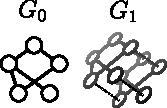
\includegraphics[scale=1.75]{wlog_regular_pentagon}
    \end{figure}

    We show by induction that each $G_i$ is triangle free, $\Delta(G_i)=\Delta(G_0)\ \forall i\in\N$
    and $\frac{P(G_i)}{|G_i|\Delta(G_i)^4} \geq \frac{P(G_0)}{|G_0|\Delta(G_0)^4}$.
    $G_0$ satisfies these conditions
    by assumption; Assume they hold for $G_i$. First we argue that $G_{i+1}$ has no
    triangles. Clearly each copy of $G_i$ has no triangles so we need to show the
    addition of edges between two 2 copies of $G_i$ doesn't induce any triangles.
    Each edge we add is between two copies of a vertex $v\in V(G_i)$. This means
    each vertex in $G_{i+1}$ has at most 1 neighbour outside of its own copy of $G_i$.
    Therefore adding an edge between two copies of some $v$ cannot induce a 3-cycle
    as the neighbourhoods of each copy of $v$ will be disjoint so $G_{i+1}$ is
    triangle free. Next we show $\Delta(G_{i+1})=\Delta(G_i)=\Delta(G_0)$; This is
    clear as we add an edge only to vertices $v$ which have $\deg v < \Delta(G_i)=\Delta(G_0)$
    meaning we do not increase the maximum degree.
    Finally we show that
    $\frac{P(G_{i+1})}{|G_{i+1}|\Delta(G_{i+1})^4} \geq \frac{P(G_0)}{|G_0|\Delta(G_0)^4}$.
    This is also easy as $|G_{i+1}|=2|G_i|$ but $P(G_{i+1}) \geq 2 P(G_i)$ as we take
    two copies of $G_i$.

    Finally we note that the minimum degree increases by 1 every iteration if the
    graph is non-regular: $\delta(G_i) < \Delta(G_i) \implies \delta(G_{i+1})=\delta(G_i) + 1$.
    Then as $\Delta(G_i)=\Delta(G_0)\forall i\in\N$ this means there can be at most
    $\Delta(G_0)-\delta(G_0) \leq \Delta(G_0)$ iterations until we arrive at a regular
    $G_k$. We found then a regular graph $G_k$ which satisfies our conditions.
\end{proof}

\begin{corollary}
    \label{corollary:pentagon_regular_suffices}
    It suffices to show that $\frac{P(G)}{|G|\Delta(G)^4} \lesssim \lambda$
    only for regular triangle free $G$.
\end{corollary}

\begin{proof}
    Assume the bound holds for regular graphs.
    Assume then for contradiction that
    there is some triangle free $\Delta$-increasing sequence $(G_k)_{k\in\N}$
    such that $\lim_{k\to\infty} \frac{P(G_k)}{|G_k|\Delta(G_k)^4} > \frac{1}{5\cdot 8}$.
    Then by the previous lemma we can construct a sequence
    $(G_k')_{k\in\N}$ where each $G_k'$ is triangle free and regular
    such that $\Delta(G_k')=\Delta(G_k)$ and
    $\frac{P(G_k')}{|G_k'|\Delta(G_k')^4} >\frac{P(G_k)}{|G_k|\Delta(G_k)^4}$
    for all $k\in\N$. Hence this is a $\Delta$-increasing triangle free regular
    sequence such that
    \[
        \limsup_{k\to\infty} \frac{P(G_k')}{|G_k'|\Delta(G_k')}
        \geq
        \lim_{k\to\infty} \frac{P(G_k)}{|G_k|\Delta(G_k)}
        > \lambda
    \]
    which is a contradiction.
\end{proof}

Now we know we only need to prove the bound asymptotically for regular graphs.
The final reduction step is the following simple lemma
\begin{lemma}
    \label{lemma:pentagon_local_count}
    Let $P(G, v)$ be the number of pentagons in $G$ containing $v$. If we have some
    $\lambda \in \R$ such that
    $\frac{P(G, v)}{\Delta(G)^4} \lesssim \lambda$ as $\Delta(G)\to\infty$
    then
    $\frac{P(G)}{|G|\Delta(G)^4} \lesssim \frac{1}{5}\lambda$ as $\Delta(G)\to\infty$.
\end{lemma}

\begin{proof}
    Note $\sum_{v\in V(G)}P(G, v) = 5P(G)$. Hence
    \begin{multline*}
        \frac{P(G)}{|G|\Delta(G)^4}
        = \frac{\sum_{v\in V(G)} P(G, v)}{5|G|\Delta(G)^4}
        = \frac{\sum_{v \in V(G)} \lambda\Delta(G)^4 + o(\Delta(G)^4)}{5|G|\Delta(G)^4}\\
        = \frac{\lambda|G|\Delta(G)^4 + o(|G|\Delta(G)^4)}{5|G|\Delta(G)^4}
        = \frac{\lambda}{5} + o(1)
    \end{multline*}
\end{proof}

Now we see how our proof of theorem \ref{thm:simple_pentagon_bound} will go.
We need only show that for a regular triangle free graphs $G$ and
$v\in V(G)$ we have an asymptotic bound of $P(G, v) \lesssim \frac{\Delta(G)^4}{8}$.
This is something that local flags can prove.

Unfortunately we know that this approach cannot be directly improved to show the
full $\frac{|G|}{5}\frac{\Delta(G)^4}{16}$ bound as this result is tight:

\begin{lemma}
    There exists regular graphs $G$ with arbitrarily large $\Delta(G)$ such that
    some $v\in V(G)$ sits on $\frac{|G|}{5}\frac{\Delta(G)^4}{8}$ 5-cycles.
\end{lemma}

\begin{proof}
    For any $k\in\N$ even we construct the following graph: Construct a blowup of the 6-cycle
    of size $k/2$. This consists of 6 independent sets of size $k/2$ which are densely
    connected to their neighbours in a 6-cycle.
    We then add a single extra vertex which will be our distinguished vertex $v\in V(G)$ and
    connect it to densely to 2 of the supernodes which are on opposite ends of the cycle.

    \begin{figure}[!ht]
        \centering
        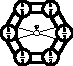
\includegraphics[scale=4]{hexagon_bound_example}
    \end{figure}

    This graph is almost regular in that every vertex has degree $k$, except those
    in the 2 supernodes connected to $v$ which have degree $k+1$. This is a detail that
    doesn't matter and could be addressed but would distract from the core of the construction.
    Asymptotically speaking this construction is regular.

    Note then that we can construct a pentagon going through $v$ by first choosing
    a vertex from each of the connected supernodes which is $\left(\frac{k}{2}\right)^2$
    choices. Then we can choose the final 2 vertices of the pentagon by either going
    "up" or "down" and picking any vertex from each of the supernodes. This gives us
    $2\left(\frac{k}{2}\right)^2$ choices leading to an overall number of
    $\frac{k^4}{8}$ 5-cycles as required.
\end{proof}

\section{Local Flags for Regular Graphs}
\label{sec:local_flags_regular_graphs}

We show now why focusing on only regular graphs is so powerful in the context of
local flags. As we saw in section \ref{sec:semidefinite_method} we want to find
interesting elements of the semantic cone $\SemCone^\emptyset$. This is dual to
finding general linear relations of density limits of local flags.

Let $\Gcl$ be a class of regular graphs.
We start by defining the extension of a flag:

\begin{definition}[Extension]
    Let $\sigma$ be a type of size $k$. Then we define the
    \textbf{extension} $\ext^\sigma_i$ as the sum of all $\sigma$ flags $\in\HeredG{}^\sigma$
    of size $k+1$ which have an edge between the unlabelled vertex the and vertex labelled $i$.
\end{definition}

\begin{note}
    By lemma \ref{lemma:local_if_connected} such flags are all local flags so
    $\ext^\sigma_i \in \Lcl^\sigma$.
\end{note}

\begin{example}
    Let $\Gcl$ be the class of red-black vertex coloured regular graphs then
    see figure \ref{fig:extension_example} for an example $\sigma$ and two possible
    extensions of $\sigma$ corresponding to extending on vertex 1 or 2.
    \begin{figure}[ht]
        \centering
        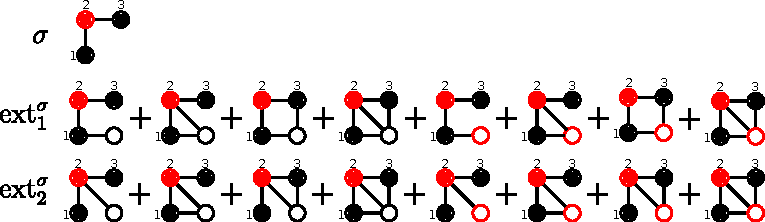
\includegraphics{extension_example}
        \caption{Example type $\sigma$ with two possible extensions}
        \label{fig:extension_example}
    \end{figure}
\end{example}

These extensions are important for the following reason:

\begin{lemma}
    If $\Gcl$ consists of only regular graphs then for any $\sigma$ and $\phi\in\Phi^\sigma$ we have
    $\phi(\ext_i^\sigma) = 1\ \forall\ i \in [|\sigma|]$.
\end{lemma}

\begin{proof}
    Let $\ext_i^\sigma=\sum_{\alpha\in I}F_\alpha$ for some index set $I$. Let
    $(G,\eta)$ be any $\sigma$-flag with $G\in\Gcl$. Then any instance of some
    $F_\alpha$ is a subset $\im\eta \subseteq U \subseteq V(G)$ where
    $G[U] \cong F_\alpha$. In particular $|U|=|F_\alpha|=|\sigma|+1=|\im\eta| + 1$ so
    $U = \im\eta \cup \{v\}$ for some $v\in V(G)$. In particular by definition of
    $\ext_i^\sigma$ this $v$ must be connected in $G$ to $\eta(i)$. Hence
    $v \in N(\eta(i))\setminus \im\eta$. This map from a copy of $F_\alpha$ in $G$ to
    a specific vertex is injective as we can
    take the $\sigma$-flag $(G[\im\eta\cup\{v\}], \eta)$ which must be isomorphic
    to $F_\alpha$. This map is also surjective for the same reason, given any
    $v\in N(\eta(i)) \setminus \im\eta$ we take $G[\im\eta \cup \{v\}$ which must
    be isomorphic to some flag $F_\alpha$ where the unlabelled vertex is connected to
    the vertex labelled $i$, so appears in the $\ext_i^\sigma$ expression.

    Therefore $\sum_{\alpha\in I}c(F_\alpha; (G,\eta)) = |N(\eta(i))\setminus\im\eta|$.
    In particular then
    \[
        \rho(\ext_i^\sigma; (G,\eta))
        = \sum_{\alpha \in I} \frac{c(F_\alpha; (G,\eta)}{\Delta(G)}
        = \frac{|N(\eta(i)) \setminus \im\eta|}{\Delta(G)}
    \]
    The size of $\im\eta$ is constant and $|N(\eta(i))|=\Delta(G)$ so this is
    in the range $[1-\frac{|\im\eta|}{\Delta(G)}, 1]$. Hence
    $\rho(\ext^\sigma_i; (G,\eta)) = 1 - o(1)$ so we do get that
    $\phi(\ext_i^\sigma)=1\ \forall\ \phi\in\Phi^\sigma$.
\end{proof}

\begin{note}
    This proof only really required that sequences of graphs in $\Gcl$ are
    \textit{asymptotically} regular so the conditions for this lemma could be relaxed
    slightly.
\end{note}

\begin{corollary}
    For any type $\sigma$ and $\phi\in\Phi^\sigma$ we
    have $\phi(\ext_i^\sigma - \ext_j^\sigma) = 0$ for all $i,j \in [|\sigma|]$
    and $\phi(f \cdot \ext_i^\sigma) = \phi(f)$ for all
    $f \in \Lcl^\sigma, i \in [|\sigma|]$.

    In particular $\ext_i^\sigma - \ext_j^\sigma$,
    $f\cdot \ext_i^\sigma - f$ and $f - f\cdot\ext_i^\sigma$ are all
    elements of the semantic cone $\SemCone^\sigma$.
\end{corollary}

\begin{corollary}
    \label{corollary:unlabel_extension}
    If $\sigma$ is a local type then for any $\phi\in\Phi^\emptyset$ we have
    $\phi(\llbracket \ext_i^\sigma - \ext_j^\sigma\rrbracket) = 0$
    for all $i,j\in [|\sigma|]$ and
    $\phi(\llbracket f \cdot \ext_i^\sigma\rrbracket) = \phi(\llbracket f \rrbracket)$
    for all $f\in\Lcl^\sigma$ and $i\in [|\sigma|]$.
\end{corollary}

\begin{proof}[Proof of Corollary \ref{corollary:unlabel_extension}]
    By the previous corollary $\ext_i^\sigma - \ext_j^\sigma$ are in the
    semantic cone $\SemCone^\sigma$ so by lemma \ref{lemma:local_pos_preserve}
    we must have $\llbracket \ext_i^\sigma - \ext_j^\sigma \rrbracket \in \SemCone^\sigma$
    so $\phi(\llbracket \ext_i^\sigma - \ext_j^\sigma\rrbracket) \geq 0$.
    The same goes for swapping $i$ and $j$ so
    $\phi(\llbracket \ext_j^\sigma - \ext_i^\sigma\rrbracket) \geq 0$
    implying $\phi(\llbracket \ext_i^\sigma - \ext_j^\sigma\rrbracket) = 0$.

    The same argument works for $\llbracket f\cdot\ext_i^\sigma \rrbracket$ and
    $\llbracket f\rrbracket$.
\end{proof}

\begin{note}
    These relations suggest that if we focused only on regular graph classes
    from the beginning we could have quotiented out the set of relations
    $\llbracket \ext_i^\sigma - \ext_j^\sigma\rrbracket$ from our vector space $\R\HeredG^\emptyset$
    to get a "cleaner" algebra. I have not verified that this is possible. If this is true
    it could theoretically enable us to generate smaller semidefinite programs but we would
    need an algorithmic way of reducing vectors over this subspace which prima facie is not
    a straightforward task.
\end{note}

The value of these results for us is twofold. Firstly this gives us a wide set of
easy to generate elements of the semantic cone which we can use in our semidefinite
program. Secondly though this property where
$\phi(\llbracket f \rrbracket)=\phi(\llbracket f \cdot \ext_i^\sigma\rrbracket)$ gives
us a way of expressing a vector in a subspace of larger flags. In particular multiplying by
$\ext_i^\sigma$ gives a vector over flags which are 1 larger than those in the original
vector. This will be very useful to us.

\section{Counting Pentagons with Local Flags}
\label{sec:counting_pentagons}

We want to use local flags to show an asymptotic bound that for any regular, triangle free
graph $G$ we have
$P(G, v) \lesssim \frac{\Delta(G)^4}{8}$ for any $v \in V(G)$.
We first reduce this to a problem on coloured graphs.

Let $\Gcl$ be the class of red-black vertex coloured graphs which are triangle free,
regular and such that for each $G\in\Gcl$ the number of black vertices
in $G$ is exactly $\Delta(G)$ and the set of black vertices in $G$ is independent.
Note then that $\HeredG$ is the same class without the regularity as all other
properties are hereditary.

Then we have the following reduction:

\begin{lemma}
    \label{lemma:brrb_suffices}
    Let $\brrb$ be the black-red-red-black path. Then for any $\lambda\in\R$
    $\frac{c(\brrb; G)}{\Delta(G)^4} \lesssim \lambda$ as
    $\Delta(G) \to \infty$ over $\Gcl$ implies $\frac{P(H, v)}{\Delta(H)^4}\lesssim\lambda$
    as $\Delta(H)\to\infty$ over the class of regular triangle free graphs.
\end{lemma}

\begin{proof}

    Let $G$ be a simple regular triangle free graph and fix some $v\in V(G)$. Then
    $|N(v)| = \Delta(G)$ and the set $N(v)$ is independent.

    Any pentagon containing $v$ then must contain 2 vertices of $N(v)$ and 2 vertices
    outside of $N(v)$. In particular if we construct a 3-vertex-coloured graph $H$
    which is a copy of $G$ where $v$ is green, $N(v)$ is black and all others are
    red then we want to count how many pentagons contain 1 green vertex, 2 black vertices
    and 2 red vertices. Then as all black vertices are connected to the green vertex it
    suffices to count how many black-red-red-black paths there are in $H$. In fact
    removing $v$ from $H$ has no effect on this count so WLOG we can remove it.

    \begin{figure}[!ht]
        \centering
        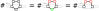
\includegraphics[scale=1.45]{pentagon_reduction}
    \end{figure}

    This $H$ graph has (up to asymptotically 0 terms) the same max degree as $G$
    so any bound on $H$ asymptotically applies to $G$.
\end{proof}

\subsection{Local Flags Setup}

We have decided on a class of graphs $\Gcl$ so we need to now find a description of
the local $\sigma$-flags.

\begin{lemma}
    \label{lemma:pentagon_local_flags}
    A $\sigma$-flag $F$ is a local $\sigma$-flag (relative to our choice of
    $\Gcl$) iff each connected component of $F$ contains a labelled vertex or a
    black vertex.
\end{lemma}

\begin{proof}
    First we show if each connected component of $F$ contains a labelled or black
    vertex then $F$ has bounded density function. We do this by induction on $|F|-|\sigma|$.
    The base case is that $|F|=|\sigma|$ which implies $F$ consists only of labelled
    vertices meaning $c(F; G) = 1 \in O(\Delta(G)^0)$ for any $G\in\Gcl^\sigma$
    as required.

    Otherwise assume $|F|>|\sigma|$. Note then that as each connected component of
    $F$ contains at least one labelled or black vertex each vertex $u$ of $F$ has a
    finite minimum distance $d(u)$ to some labelled or black vertex (where
    $d(u)=0$ for all black and labelled $u$ and $d(u) > 0$ for all unlabelled red vertices).
    Let $v$ be some unlabelled vertex in $F$ with maximum $d(v)$. Consider then removing $v$ from
    $F$: $F' := F[V(F)\setminus \{v\}]$. This $F'$ must not have any connected
    components with no black or labelled vertices because we chose $d(v)$ large as
    possible. Hence $c(F'; G) \in O\left(\Delta(G)^{|F|-|\sigma|-1}\right)$ by our
    induction hypothesis.

    Consider then some subset $\im\eta\subseteq U' \subseteq V(G)$ such that
    $G[U'] \cong F'$. We want to bound how many copies $U$ of $F$ can we obtain
    by adding one more vertex $u\in V(G)$ onto which our removed $v$ can be mapped.
    There are 2 cases: If the $v\in V(F)$ we removed was a black vertex then
    $u$ must be a black vertex, there are only $\Delta(G)$ of those meaning there
    are $\leq \Delta(G)$ possible such $U$'s. Otherwise $v$ was a red vertex
    meaning it was connected to $V(F)\setminus\{v\}$. This means $u$ must be
    in the neighbourhood of one of the vertices of $U$ of which there are
    $O(\Delta(G))$ such options. In either case there are only $O(\Delta(G))$ such
    extensions of $U'$.
    In particular though every copy $U$ of $F$ can be reached in this way. This is easily
    seen by taking any such copy and removing the vertex $u$ that $v$ is mapped to, this must
    give you a copy $U'$ of $F'$ with which we can re-add $u$ to get back to $U$.
    Therefore this process counts all copies $U$ of $F$ in $G$ giving us a bound of
    $c(F'; G) \cdot O(\Delta(G)) = O\left(\Delta(G)^{|F|-|\sigma|}\right)$ as required.

    Now that we know any such $F$ has bounded density function we simply note that
    any label extension of $F$ gives you a new flag which also has a labelled or
    black vertex in each connected component. Therefore label extension preserves
    bounded density functions so $F$ is a local $\sigma$-flag.

    We also show that this encapsulates all local $\sigma$-flags. This isn't strictly
    required for our application so I give a brief idea of the proof. Taking any
    flag with a connected component consisting of all unlabelled red vertices we can
    easily construct a sequence of graphs $(G_k)_{k\in\N}$ in $\Gcl$ where we keep
    increasing the number of copies of the unlabelled red component. We can do this maintaining
    the fact that each $G_k$ is regular and has only $\Delta(G)$ black vertices. Then
    the number of copies of $F$ increases unbounded along this sequence proving $F$ is not
    local.
\end{proof}

Now that we know our set of local flags, which tells us our local types by
lemma \ref{lemma:local_type_equiv} we can now formulate our problem as a semidefinite
problem.

\section{The Semidefinite Program}
\label{sec:pentagon_sdp}

We fixed our class of graphs $\Gcl$ to be the class of red-black vertex coloured
regular triangle-free graphs with $\Delta(G)$ black vertices such that the set of
black vertices is independent.
We want to asymptotically bound the number of black-red-red-black paths in this
class. This means we have the following objective function: $\brrb$.
This is a local flag by lemma \ref{lemma:pentagon_local_flags}. We will now use
the semidefinite method (Section \ref{sec:semidefinite_method}) to find a bound
$\lambda\in\R$ such that $\phi(\brrb)\leq \lambda\ \forall\ \phi\in\Phi^\sigma$.

\begin{note}
    It proves to be more intuitive to describe our problem in terms of maximising
    $\phi(\brrb)$. We then use duality (section \ref{sec:sdp_duality}) to convert
    this to a problem of finding some $\lambda\emptyset - \brrb\in\SemCone^\emptyset$
    which proves the $\lambda$ upper bound rigorously.
\end{note}

We need to pick a subspace of $\Lcl^\emptyset$ to optimise our objective
function over. A standard method (e.g. \cite{grzesikFlagAlgebrasExtremal2014},
\cite{cummingsMonochromaticTrianglesThreecoloured2013}) is picking the subspace spanned by flags
of some fixed size. In this case it suffices to consider the subspace of flags of
size 5.\footnote{Picking larger flags intuitively allows the search to find tighter bounds but
comes at the cost of computation time}.

By our choice of subspace we need to find a vector $f$ over flags of size 5 such that
bounding $\phi(f)$ gives a bound on $\phi(\brrb)$. To achieve this we view
$\brrb$ as a $\brrb$-flag in itself: $\brrbmarked$.
Letting $\sigma=\brrb$ we note that $\sigma$ is a local type and we can compute
$\llbracket \brrbmarked \rrbracket=\frac{2}{4!}\brrb = \frac{1}{12}\brrb$.
We can then compute $\ext_1^\sigma$ and then use corollary \ref{corollary:unlabel_extension}
which tells us that
\[
    \frac{1}{12}\phi(\brrb) = \phi(\llbracket \brrbmarked \rrbracket)
    = \phi(\llbracket \brrbmarked \cdot \ext_1^\sigma\rrbracket).
    = \phi(\llbracket \ext_1^\sigma\rrbracket).
\]
where we used that $\sigma$ is the unit of the algebra $\Lcl^\sigma$. Then
$\ext_1^\sigma$ is a vector of flags of size 5: See figure \ref{fig:pentagon_objective}.
It suffices then to try to maximise $\llbracket \ext_1^\sigma\rrbracket$: Call this
vector $O$.

\begin{figure}[ht]
    \centering
    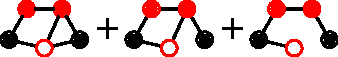
\includegraphics{pentagon_objective}
    \caption{$\ext^\sigma_1$ where $\sigma=\brrb$}
    \label{fig:pentagon_objective}
\end{figure}

To apply our semidefinite method we first need a list of known elements of the
semantic cone $\SemCone^\emptyset$ or dually a list of linear constraints on limit functionals.
For any type $\sigma$ we immediately get the elements
$\llbracket \ext^\sigma_i - \ext_j^\sigma\rrbracket$ from corollary
\ref{corollary:unlabel_extension}. We want only those that are in the subspace of
flags of size 5 so we take all such vectors where $|\sigma|=4$.

We know that in any $G\in\Gcl$ the set of black vertices is independent and has size
$\Delta(G)$. Let $B_k$ be the $\emptyset$-flag consisting of $k$ independent black
vertices. e.g. $B_1=\vertex, B_2=\nonedge, B_3=\triangleempty,\dots$. Then we know $c(B_k; G) = \binom{\Delta(G)}{k}$
for any $G\in\Gcl$ which implies $\phi(B_k)=1\ \forall\ \phi\in\Phi^\emptyset\ \forall\ k\in\N$.
We would like to add these to the list of constraints. For $k=5$ this is already in
the subspace of flags of size 5 so we can add it directly. For $k < 5$ we need
to do the same extension trick as with our objective function where we use that
$\llbracket B_k \rrbracket = B_k$ to get
\begin{multline*}
    1 = \phi(B_k)=\phi(\llbracket B_k \rrbracket)
    = \phi(\llbracket B_k \cdot \ext_1^{B_k}\rrbracket)
    = \phi\left(\left\llbracket B_k \cdot \left(\ext_1^{B_k}\right)^{5-k}\right\rrbracket\right)\\
    = \phi\left(\left\llbracket \left(\ext_1^{B_k}\right)^{5-k}\right\rrbracket\right).
\end{multline*}
$\left(\ext_1^{B_k}\right)^{5-k}$ is a vector over flags of size 5 so this is
a constraint we can use.

Finally then we want to encode constraints of the form $\phi(\llbracket f^2 \rrbracket) \geq 0$
for all $f\in \Lcl^\sigma$. To do this we need to find local types $\sigma$ and sizes $n$
such that $f^2$ is an expression of flags of size 5 for all $f\in\Glocn^\sigma$.
Those pairs $(\sigma, n)$ are ($\vertex$, $3$), ($\triangleempty$, $4$), ($\pentsqtypeone$, $4$),
($\pentsqtypetwo$, $4$), ($\pentsqtypethree$, $4$), and ($\pentsqtypefour$, $4$).

Let $\Bcl=(F_1, \dots, F_\ell)$ be the basis of all flags of size 5.
In summary then our problem is:
\begin{align*}
    \max_{x\in\R^\ell}\ \ &\ \phi_x(O)\\
    \text{such that}\ \ &\ \phi_x(F_i) \geq 0\ \forall\ i \in [\ell]\\
    &\ \phi_x(\llbracket \ext^\sigma_i - \ext^\sigma_j\rrbracket) = 0\ \forall\
    |\sigma|=4, i, j \in [4]\\
    &\ \phi_x(B_5) = 1\\
    &\ \phi_x\left(\left\llbracket\left(\ext_1^{B_k}\right)^{5-k}\right\rrbracket\right) = 1\
    \forall\ k \in [4]\\
    &\ \phi_x(\llbracket f^2 \rrbracket) \geq 0 \forall f \in \Lcl_n^\sigma\ \forall (\sigma, n)
    \ \text{from above list}.
\end{align*}

We know from section \ref{sec:semidefinite_method} how to construct the corresponding
SDP. A solution to this SDP finds a convex combination of elements of the semantic cone
which prove an upper bound on $\phi(O)\ \forall\ \phi\ \in \Phi^\emptyset$.

We use a SDP solver to show the following result:
\begin{lemma}
    \label{lemma:pentagon_1_4_bound}
    \[
        \frac{1}{4}\emptyset - O \in \SemCone^\emptyset.
    \]
\end{lemma}
In the next section (\ref{sec:pentagon_proof_validation}) we will show how we make this
SDP solution rigorous. For now we show that this bound suffices to prove theorem
\ref{thm:simple_pentagon_bound}.

\begin{proof}[Proof of theorem \ref{thm:simple_pentagon_bound}]
    By lemma \ref{lemma:pentagon_1_4_bound} we have that
    $\phi(O) \leq \frac{1}{4}\ \forall\ \phi\in\Phi^\sigma$.
    We know that $\frac{1}{12}\phi(\brrb)=\phi(O)$ so $\phi(\brrb) \leq 3$.
    Therefore for any $\Delta$-increasing sequence of graphs $(G_k)_{k\in\N}$ we have
    $\lim_{k\to\infty} \frac{c(\brrb; G_k)}{\binom{\Delta(G_k)}{4}} \leq 3$.
    Intuitively then $\binom{\Delta(G_k)}{4}$ is asymptotically $\frac{\Delta(G_k)^4}{4!}$ so
    we get $\lim_{k\to\infty} c(\brrb; G_k) \leq \frac{3}{4!} = \frac{1}{8}$.
    We show this argument more precisely now:

    We use the fact that
    $\frac{\Delta(G_k)!}{(\Delta(G_k)-4)!} = \Delta(G_k)^4 + o(\Delta(G_k)^4)$
    to show that
    \[
        \begin{split}
            \lim_{k\to\infty}\frac{c(\brrb; G_k)}{\Delta(G_k)^4}
            &= \lim_{k\to\infty}\frac{c(\brrb; G_k)}{\binom{\Delta(G_k)}{4}}
            \frac{\Delta(G_k)!}{4!(\Delta(G_k)-4)!\Delta(G_k)^4}\\
            &= \lim_{k\to\infty}\frac{c(\brrb; G_k)}{\binom{\Delta(G_k)}{4}}
            \frac{\Delta(G_k)^4 + o(\Delta(G_k)^4}{4!\Delta(G_k)^4}\\
            &= \lim_{k\to\infty}(1+o(1))\frac{1}{4!}\frac{c(\brrb; G_k)}{\binom{\Delta(G_k)}{4}}\\
            &\leq \frac{1}{8}.
        \end{split}
    \]
    Then by lemma \ref{lemma:brrb_suffices}
    $\frac{P(G, v)}{\Delta(G)^4}\lesssim \frac{1}{8}$ for any regular triangle free
    $G$ and $v \in V(G)$.
    Lemma \ref{lemma:pentagon_local_count} tells us then
    $\frac{P(G)}{|G|\Delta(G)^4}\lesssim \frac{1}{5\cdot 8}$ for any regular triangle
    free $G$. Corollary \ref{corollary:pentagon_regular_suffices} shows that
    we can drop the regular requirement.
    Finally then lemma \ref{lemma:pentagon_asymp_suffices} shows that this
    asymptotic bound implies the non-amsymptotic bound.
    \[
        \therefore P(G) \leq \frac{|G|}{5}\frac{\Delta(G)^4}{8}
        \ \forall\ G\ \text{triangle free}.
    \]
\end{proof}

\section{SDP Proof Validation}
\label{sec:pentagon_proof_validation}

We've shown in the previous section how to express our problem in the form of a
semidefinite program and we claimed that SDP software found a solution proving a bound
of $1/8$. Clearly though appealing to a software implementation, no matter how well tested,
is not rigorous. We saw in section \ref{sec:semidefinite_method} how such an SDP
solution corresponds to constructing a specific element of the semantic cone by taking
convex combinations of known elements of the cone. In this section we will show the
combination of elements that was found by the SDP software, verifying that it is indeed
a valid proof.

We will defer the specific details of how we converted the SDP solution into the following
proof to TODO (appendix?).

First, as a reminder we were trying to bound $\phi(O)=\frac{1}{12}\phi(\brrb)$
where we defined $O$ as an extension of $\sigma_O = \brrb$:
$O = \llbracket \ext_1^{\sigma_O}\rrbracket.$ We expand this and find that
\[
    O = \frac{1}{60}\pentF{9} + \frac{1}{120}\pentF{37} + \frac{1}{60}\pentF{55}
\]
For convenience we scale this by 120 to get
$2\pentF{9} + \pentF{37} + 2\pentF{55}$. Then we prove that
$120\phi(O) \leq\lambda\ \forall\ \phi\in\Phi^\emptyset$ by showing
$\lambda\emptyset - 2\pentF{9} + \pentF{37} + 2\pentF{55}\in\SemCone^\emptyset$.

First we take $B_1=\vertex$ as defined above. We know
$1=\phi(\vertex)=\phi(\llbracket (\ext^\vertex_1)^4 \rrbracket) = \frac{1}{5}\phi(\pentF{6})$
for all $\phi\in\Phi^\emptyset$ hence 
\begin{equation}
    5\emptyset - \pentF{6} \in\SemCone^\emptyset.
    \label{eq:pent_b1}
\end{equation}

Next, by corollary \ref{corollary:unlabel_extension} for any local type $\sigma$
and $i,j \in [|\sigma|]$ and we have
$\llbracket \ext_i^\sigma - \ext_j^\sigma\rrbracket\in\SemCone^\emptyset$. It also
proves easier to scale these by $120$ as with $O$.
We compute some such vectors for the following fixed types:
$\sigma_1 := \pentsig{1}, \sigma_2 := \pentsig{2}$,
$\sigma_3 := \pentsig{3}$, $\sigma_4 := \pentsig{4}$
and $\sigma_5 := \pentsig{5}$.
\begin{align}
    120\llbracket \ext_2^{\sigma_1} - \ext_1^{\sigma_1} \rrbracket
    &=-4\pentF{4} - 6\pentF{5} + 2\pentF{12} + 2\pentF{24} + 4\pentF{32}
    \in\SemCone^\emptyset.\label{eq:pent_sig_1}\\
    120\llbracket \ext_1^{\sigma_2} - \ext_2^{\sigma_2} \rrbracket
    &= 
    24\pentF{6} - 4\pentF{13} - 4\pentF{15} - 2\pentF{18} - 2\pentF{25} - 12\pentF{33} - 6\pentF{34}
    \in \SemCone^\emptyset.\label{eq:pent_sig_2}\\
    120\llbracket \ext_2^{\sigma_3} - \ext_1^{\sigma_3} \rrbracket
    &=2\pentF{11} + \pentF{12} - 2\pentF{15} + \pentF{22} + 2\pentF{24} - 2\pentF{25}
    \label{eq:pent_sig_3}.\\
    120\llbracket \ext_2^{\sigma_4} - \ext_1^{\sigma_4} \rrbracket
    &= \pentF{8} + \pentF{12} - 2\pentF{15} + 4\pentF{31} + 4\pentF{32} - 6\pentF{34}
    \label{eq:pent_sig_4}.\\
    120\llbracket \ext_3^{\sigma_5} - \ext_1^{\sigma_5} \rrbracket
    &= -2\pentF{16} - \pentF{17} + \pentF{37} + 2\pentF{55}
    \label{eq:pent_sig_5}.
\end{align}

Now we can take a convex combination of these elements of the semantic cone to
get another element of the semantic cone.
\begin{multline}
    6\cdot (\ref{eq:pent_b1})
    + 1\cdot (\ref{eq:pent_sig_1})
    + \frac{1}{4} \cdot (\ref{eq:pent_sig_2})
    + 1\cdot (\ref{eq:pent_sig_3})
    + 1\cdot (\ref{eq:pent_sig_4})
    + 2\cdot (\ref{eq:pent_sig_5})\\
    =
    30\emptyset -4\pentF{4} - 6\pentF{5} + \pentF{8} + 2\pentF{11} + 4\pentF{12} - \pentF{13} -
        5\pentF{15} - 4\pentF{16} - 2\pentF{17} - \frac{1}{2}\pentF{18}\\
        + \pentF{22} + 4\pentF{24} - \frac{5}{2}\pentF{25} + 4\pentF{31} + 8\pentF{32} - 3\pentF{33}
        - \frac{15}{2}\pentF{34} + 2\pentF{37} + 4\pentF{55}.
    \label{eq:pent_lin_sum}
\end{multline}

Consider then the type $\sigma_6=\pentsig{6}$ and the following
vectors $f,g \in \Lcl^{\sigma_6}$.
\[
    f = -\pentcf{0}{3} + \frac{1}{4}\pentcf{0}{4} + \frac{1}{4}\pentcf{0}{5}+\frac{1}{2}\pentcf{0}{6}
    \ \ \ \ g = -\frac{1}{4}\pentcf{0}{4} + \frac{1}{4}\pentcf{0}{5}
\]
Then by \ref{lemma:local_pos_preserve} both of the following are elements of the
semantic cone:
\[
    \begin{split}
        120 \llbracket f^2 \rrbracket &= 
    4\pentF{4} - \pentF{8} - 2\pentF{11} + \pentF{13} + \frac{1}{4}\pentF{18} - \pentF{22} -
        4\pentF{31} + 3\pentF{33} + \frac{1}{4}\pentF{40} + \frac{1}{4}5\pentF{55}\\
        120 \llbracket g^2 \rrbracket &= 
        \frac{1}{4}\pentF{18} - \frac{1}{4}\pentF{40} - \frac{1}{4}\pentF{55}
    \end{split}
\]
The sum of these two elements gives a new element of the semantic cone
\begin{equation}
    4\pentF{4} - \pentF{8} - 2\pentF{11} + \pentF{13} + \frac{1}{2}\pentF{18} - \pentF{22} -
    4\pentF{31} + 3\pentF{33} \in \SemCone^\emptyset
    \label{eq:pent_cs_0}
\end{equation}

We do the same thing with the type $\sigma_7 := \pentsig{7}$: Take the following
vectors $h, \ell \in \Lcl^{\sigma_7}$.
\[
    h = -\frac{1}{2}\pentcf{1}{4} - \pentcf{1}{5} + \frac{1}{2}\pentcf{1}{7}
    \ \ \ \ \ell = \pentcf{1}{3} - \pentcf{1}{4} + \pentcf{1}{5} - \pentcf{1}{7}
\]
Then we can compute
\[
    \begin{split}
        120 \llbracket h^2 \rrbracket &= 
        -2\pentF{9} + \pentF{15} + 2\pentF{16} + \frac{1}{2}\pentF{25} + \frac{3}{2}\pentF{34} -
        \pentF{37} - 2\pentF{55}\\
        120 \llbracket g^2 \rrbracket &= 
        6\pentF{5} - 4\pentF{12} + 4\pentF{15} + 2\pentF{16} + 2\pentF{17} - 4\pentF{24} + 2\pentF{25} - 8\pentF{32}\\
        &\ \ \ + 6\pentF{34} - 2\pentF{37} - 4\pentF{55}.
    \end{split}
\]
The sum of these two elements of the semantic cone is:
\begin{multline}
    6\pentF{5} - 2\pentF{9} - 4\pentF{12} + 5\pentF{15} + 4\pentF{16} + 2\pentF{17} - 4\pentF{24} + \frac{5}{2}\pentF{25} - 8\pentF{32}\\
    + \frac{15}{2}\pentF{34} - 3\pentF{37} - 6\pentF{55}
    \in\SemCone^\emptyset
    \label{eq:pent_cs_1}
\end{multline}

Finally then we take the combination of equations \ref{eq:pent_lin_sum}, \ref{eq:pent_cs_0}
and \ref{eq:pent_cs_1} to get our final element of the cone.
\[
    (\ref{eq:pent_lin_sum}) + (\ref{eq:pent_cs_0}) + (\ref{eq:pent_cs_1})
    = 30\emptyset -2\pentF{9} - \pentF{37} - 2\pentF{55}
    \in\SemCone^\emptyset
\]
We know $120O = 2\pentF{9} + \pentF{37} + 2\pentF{55}$ so
$30\emptyset - 120O \in \SemCone^\emptyset$. This implies
$\frac{1}{4}\emptyset - O \in \SemCone^\emptyset$ as required.
This proves lemma \ref{lemma:pentagon_1_4_bound} completing our proof
of theorem \ref{thm:simple_pentagon_bound}.

\section{Proving the Stronger Result}
\label{sec:pentagon_stronger}

We can use local flags in a more complex way to get the stronger result
of theorem \ref{thm:full_pentagon_bound}. This approach is originally an idea from Eoin Hurley.

To prove the bound in theorem \ref{thm:simple_pentagon_bound} we defined
$P(G,v)$ to be the number of pentagons containing a $v \in G$
and used local flags find an upper bound.
To prove the strong result in theorem \ref{thm:full_pentagon_bound}
we will bound the following function. For fixed $v\in G$ define
\[
    Q(G, v) := \Delta(G)P(G, v) 
    + \sum_{u \in N(v)}P(G, u).
\]

Then we claim
\begin{lemma}
    \label{lemma:pent_q_v}
    For $G$ triangle free and $v\in V(G)$
    \[
        Q(G, v) \lesssim 0.2073 \Delta(G)^5
        \ \text{as}\ \Delta(G) \to\infty
    \]
\end{lemma}

We will prove this lemma now using local flags.
We use the same class of graphs $\Gcl$ as before, where the black vertices represent
those in the neighbourhood of $v$ and the others are red.
We've seen already then how to convert a triangle free regular graph $G$ into
the corresponding $G' \in \Gcl$ such that $\rho(\brrb, G) = P(G,v)/\binom{\Delta(G)}{4}$.

Note that any pentagon passing through the neighbourhood of $v$ contains at most 2
such vertices. Therefore
\[
    \rho(\pentF{56} + 2\pentF{55}; G')
    = \frac{\sum_{u \in N(V)} P(G, v)}{\binom{\Delta(G)}{5}}.
\]
Now we use the same extensions trick from before to embed our desired vector
into a space of flags of size $n$ and get the following objective vector
\[
    O := \llbracket \brrbmarked \cdot (\ext^{\sigma_1}_1)^{n-4} \rrbracket
    + \llbracket \pentF{56marked} \cdot (\ext^{\sigma_2}_1)^{n-5} \rrbracket
    + 2\llbracket \pentF{55marked} \cdot (\ext^{\sigma_3}_1)^{n-5} \rrbracket
\]
where $\sigma_1=\brrb, \sigma_2=\pentF{56}, \sigma_3=\pentF{55}$.
Then using the exact same set of constraints as from section 
\ref{sec:pentagon_sdp} we can use an SDP solver using flags of size $n=8$ to find:
\begin{lemma}
    \[
        0.4146\emptyset - O \in \SemCone^\emptyset
    \]
    hence $\phi(O) \leq 0.4146\ \forall\ \phi\in\Phi^\emptyset$.
\end{lemma}
Calculating the normalising factors (definition \ref{def:averaging_normalisation})
we find this implies
\[
    \frac{2}{4!}\phi(\brrb) + \frac{2}{5!}\phi(\pentF{56} + 2\pentF{55}) \leq 0.4146
\]
Hence for any convergent $\Delta$-increasing sequence of graphs $(G_k)_{k\in\N}$
we have
\[
    \begin{split}
        \lim_{k\to\infty}\frac{2}{4!}\rho(\brrb; G_k)
        + \frac{2}{5!}\rho(\pentF{56}; G_k) + \frac{4}{5!}\rho(\pentF{55}; G_k)
        \leq 0.4146\\
        \implies
        \lim_{k\to\infty}\frac{2}{4!}\frac{c(\brrb; G_k)}{\binom{\Delta(G_k)}{4}}
        + \frac{2}{5!}\frac{c(\pentF{56}; G_k)}{\binom{\Delta(G_k)}{5}}
        + \frac{4}{5!}\frac{c(\pentF{55}; G_k)}{\binom{\Delta(G_k)}{5}}
        \leq 0.4146\\
        \implies
        \lim_{k\to\infty}2\frac{c(\brrb; G_k)}{\Delta(G_k)^4}
        + 2\frac{c(\pentF{56}; G_k)}{\Delta(G_k)^5}
        + 4\frac{c(\pentF{55}; G_k)}{\Delta(G_k)^5}
        \leq 0.4146\\
        \implies
        \lim_{k\to\infty} \frac{c(\brrb; G_k)}{\Delta(G_k)^4}
        + \frac{c(\pentF{56}; G_k)}{\Delta(G_k)^5}
        + 2\frac{c(\pentF{55}; G_k)}{\Delta(G_k)^5}
        \leq 0.2073
    \end{split}
\]
Therefore
\[
    \Delta(G)c(\brrb; G)
    + c(\pentF{56}; G)
    + 2c(\pentF{55}; G)
    \lesssim 0.2073\Delta(G)^5
\]
By construction though this proves the same bound holds for the $Q(G,v)$ function
\[
    \Delta(G)P(G, v)
    + \sum_{u \in N(V)}P(G, u)
    \lesssim 0.2073\Delta(G)^5
    \implies
    Q(G, v) \lesssim 0.2073\Delta(G)^5
\]
proving lemma \ref{lemma:pent_q_v}.

Now we can prove the full result of theorem \ref{thm:full_pentagon_bound}.
\begin{proof}[Proof of \ref{thm:full_pentagon_bound}]
    For a triangle-free regular graph $G$ we sum $Q(G, v)$ over all $v \in V(G)$:
    \[
        \begin{split}
        \sum_{v \in V(G)} Q(G,v)
            &= \sum_{v \in V(G)} \Delta(G)P(G, v) + \sum_{u \in N(V)}P(G, u)\\
            &= 5\Delta(G)P(G) + \sum_{v\in V(G)}\sum_{u \in N(V)}P(G, u)
        \end{split}
    \]
    Then as $G$ is regular we this comes out to
    \[
        \begin{split}
            \sum_{v \in V(G)} Q(G,v)
            &= 5\Delta(G)P(G) + \Delta(G)\sum_{u\in V(G)}P(G, u)\\
            &= 5\Delta(G)P(G) + 5\Delta(G)P(G)\\
            &= 10\Delta(G)P(G)
        \end{split}
    \]
    Therefore
    \[
        10\Delta(G)P(G) \lesssim 0.2073|G|\Delta(G)^5
        \implies P(G) \lesssim 0.02073|G|\Delta(G)^4
    \]
\end{proof}
